\chapter{Les périphériques et leur gestion par interruption}
\label{chap:interrupions}

\section{Les périphériques d'entée/sortie}


\subsection{Quelques exemples de périphériques}

Nous ne nous sommes intéressés jusqu'à maintenant qu'à l'architecture interne du microprocesseur. L'ordinateur est également constitué de périphériques pour imprimer, écouter de la musique, afficher des images, ... La figure \ref{fig:peripherique} représente une vue éclatée de l'ordinateur avec différents périphériques.

\begin{figure}[htbp]
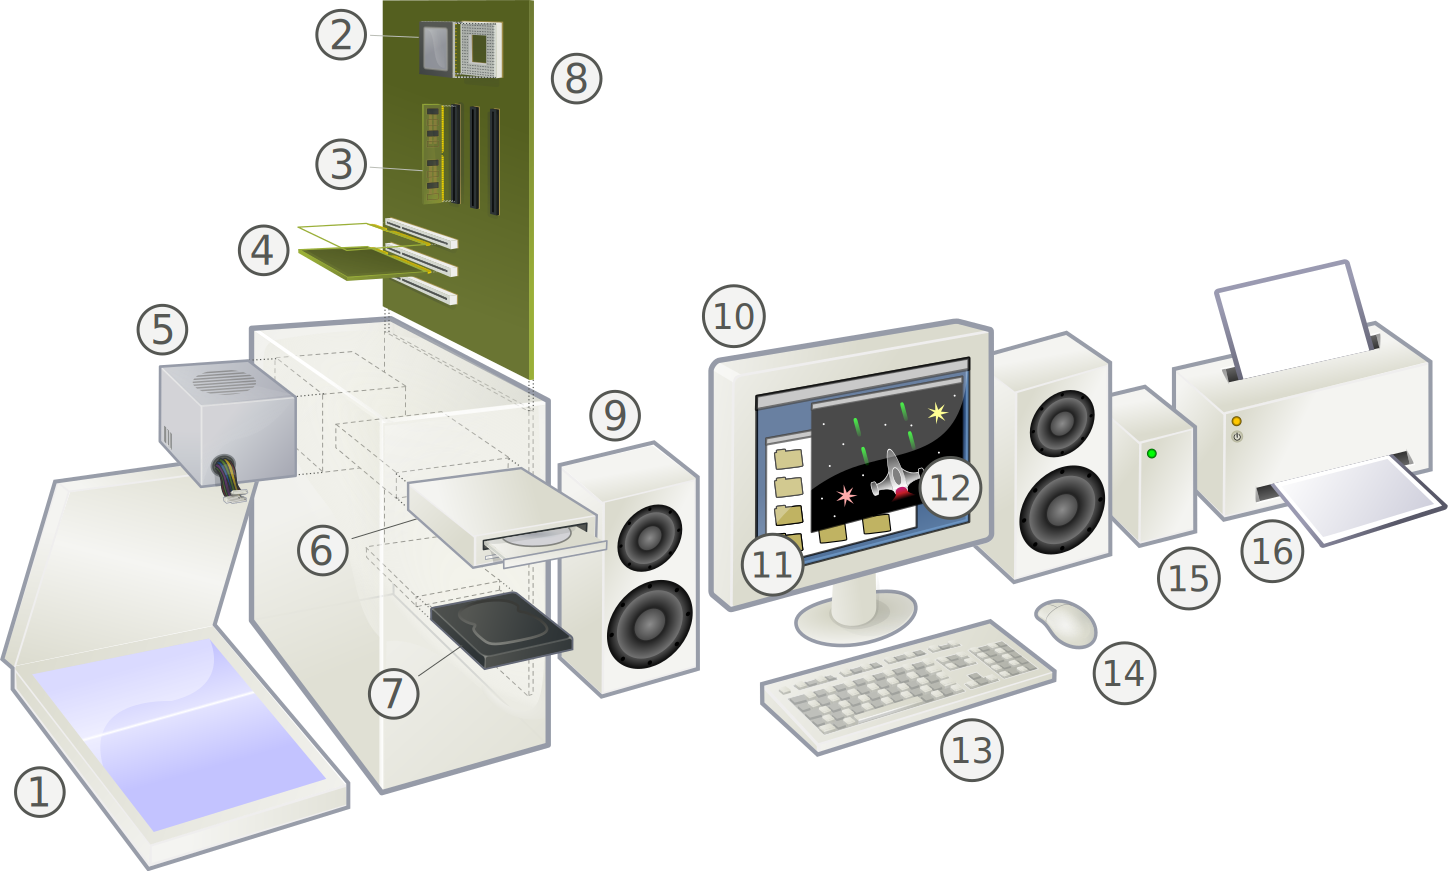
\includegraphics[width=\linewidth]{Figs/peripherique.pdf}
\caption{\label{fig:peripherique}Vue éclatée d'un ordinateur avec le microprocesseur (2), la RAM (3) enfichés sur la carte mère (8). Des cartes d'extensions (4), comme des cartes graphique, cartes son, .., sont également enfichées sur la carte mère. Différents périphériques sont connectés à l'ordinateur comme un scanner (1), un lecteur/graveur DVD (6), un disque dur (7), un écran (10), des enceintes (9), une souris (14), un clavier (13), une imprimante (16). Source : wikipedia.org}
\end{figure}


\subsection{Connexions entre le processeur et les périphériques}

La communication entre le processeur et les périphériques se fait grâce à des bus qui sont, essentiellement une collection de piste et, on va le voir, de quelques composants permettant de gérer plusieurs périphériques sur les mêmes bus. On a déjà vu quelques bus internes au microprocesseur connectés à l'UAL et aux registres. D'autres bus, les bus externes, connectent le micro-processeur aux périphériques comme représenté schématiquement sur la figure \ref{fig:chemin_peripherique}.

\begin{figure}[htbp]
\includegraphics[width=\linewidth]{Figs/chemin_peripherique.pdf}
\caption{\label{fig:chemin_peripherique} Le microprocesseur dialogue avec les périphériques grâce à des bus externes. On distingue généralement le bus de données, d'adresses et de contrôle.}
\end{figure}

La figure \ref{fig:buses} illustre une organisation type de la communication entre le microprocesseur et les différents périphériques que sont la mémoire, la carte graphique, carte réseau, disques durs, ... Cet enchevêtrement de bus est apparu au cours de l'histoire de l'informatique poussé par le besoin de meilleures performances (comme l'introduction des bus AGP pour les cartes graphiques) mais également motivé par la nécessité de maintenir une compatibilité ascendante avec des périphériques existants avant l'introduction de nouveaux bus. 

Regardons de plus près le cas des cartes graphiques. Dans les années 1980, le standard était le bus ISA. Le bus ISA permet de transporter des données sur 8 à 16 bits à des fréquences de 4 à 8 MHz, soit une bande passante d'au maximum 15 Mo/s. Il s'est avéré que ce bus ne permettait plus d'assurer une bande passante suffisante pour transporter des données à afficher sur un écran. Si on part sur un affichage à 25 images par secondes, avec des images de 1024 x 768 pixels $\approx$ 800000 pixels, chaque pixel étant disons codés sur 3 fois 8 bits (255 niveaux pour chaque composante rouge, vert, bleu, ce qui est pauvre), on atteint des besoins de bande de passante de l'ordre de 60 Mo/s. Si les données sont stockées sur le disque dur, elles doivent être transportées vers la carte graphique, et le besoin de bande passante est alors doublé. Le bus ISA ne permet pas d'atteindre de telles performances, le bus PCI est alors apparu. Celui-ci apporte une largeur de bus plus importante (32 - 64 bits) et les échanges s'y font à une fréquence plus élevée, de l'ordre de 30 à 60 MHz, que sur le bus ISA, donc une bande passante maximale de l'ordre de 500 Mo/s. Les besoins toujours plus importants des affichages vidéos ont conduit ensuite à l'introduction du bus AGP (puis AGP2X, AGP4x) qui permet d'obtenir des bandes passantes maximale de 1 Go/s. On trouve aussi maintenant des bus PCI-express qui offre des bandes passantes\footnote{\url{https://en.wikipedia.org/wiki/List_of_device_bit_rates}} de quelques Go/s. Le tableau ci-dessous donne quelques ordres de grandeurs de bande passante de bus.

\begin{tabular}{ccccc}
Bus & Largeur du bus (bits)  & Horloge (MHz) & Bande passante (Mo/s)& Année\\
\hline
ISA 16 & 16  & 8.33 & 15.9 & 1984\\
PCI 32 & 32  & 33 & 125& 1993\\
AGP & 32	&66	&250 & 1997\\
PCI Express 3 (x16) & 16 & 8000 & 16000 & 2011
\end{tabular}

Les bus ISA, PCI et AGP sont des bus parallèles, transmettant des mots complets à chaque cycle. En pratique, des problèmes techniques apparaissent lorsque les fréquences des échanges augmentent, problème qui sont moins présents sur des interfaces séries comme le bus PCI express qui autorise des fréquences d'échange bien plus élevées même si le nombre de bit échangé à chaque cycle d'horloge est moins important.
 
Les périphériques nécessitant une grande bande passante sont placés près du microprocesseur puis quelques ponts (\emph{bridge}) assurent l'interface entre les différents types de bus. Les périphériques comme la souris ou le clavier sont par exemple placés sur les bus lents contrairement à la mémoire ou la carte graphiques placées sur un bus rapide.

\begin{figure}[htbp]
\includegraphics[width=\linewidth]{Figs/buses.pdf}
\caption{\label{fig:buses} Pour supporter des périphériques disposant de différentes interfaces et nécessitant différentes performances (e.g. cartes graphiques vs disque dur), les périphériques et le microprocesseur sont interconnectés par différents niveaux de bus.}
\end{figure}

La communication sur un bus peut se faire de deux manière : synchrone ou asynchrone. La communication synchrone base les échanges sur un signal d'horloge. Prenons comme exemple une demande de lecture mémoire initiée par le processeur. La figure \ref{fig:sync_comm} illustre un échange synchrone entre un processeur et la mémoire lors d'une opération de lecture.

\begin{figure}[htbp]
\includegraphics[width=0.75\linewidth]{Figs/sync_comm.pdf}
\caption{\label{fig:sync_comm} Illustration d'une lecture mémoire initiée par le processeur avec un protocole d'échange synchrone. Les changements d'état des signaux de contrôle n'ont lieu qu'aux instants de changement d'état d'un signal d'horloge. On a ici supposé que les changements d'état n'avait lieu que sur des fronts montants d'horloge.}
\end{figure}


Lors d'un échange synchrone, les changements d'état des différents signaux ont lieu avec des changement d'état du signal d'horloge. Le processeur commence par placer l'adresse du mot mémoire à lire sur le bus d'adresse (Adr) et indique qu'il souhaite effectuer une lecture (READ), sur le module mémoire. La mémoire, voyant en entrée la requête de lecture, peut commencer à récupérer le mot mémoire demandé. Le travail de la mémoire peut prendre un peu de temps et indique au processeur, par un signal d'attente (WAIT), que les données ne sont pas encore disponibles. Après éventuellement quelques cycles d'horloge, les données sont placées par la mémoire sur le bus de données et elle indique au processeur que les données sont disponibles en désactivant le signal d'attente (WAIT). Le processeur réagit en lisant les données placées sur le bus de données et en désactivant sa requête de lecture. La principale caractéristique d'une communication synchrone est justement la synchronie, c'est à dire que tout les échanges sont rythmés par une horloge : même si la mémoire place les données sur le bus de données pendant un cycle d'horloge, le processeur ne les prendra en compte qu'au prochain tick d'horloge.

\begin{figure}[htbp]
\includegraphics[width=\linewidth]{Figs/async_comm.pdf}
\caption{\label{fig:async_comm} Illustration d'une lecture mémoire initiée par le processeur avec un protocole d'échange asynchrone. Le maître (processeur) et l'esclave (la mémoire) se verrouille mutuellement par l'intermédiaire des signaux de contrôles Msyn et Ssyn indépendemment d'une quelconque horloge.}
\end{figure}

Une communication asynchrone ne fait reposer ses échange sur aucun signal d'horloge mais sur des signaux de contrôle. On distingue généralement un maître et un esclave dans une transaction. Dans notre exemple d'une lecture mémoire, le processeur serait le maître et la mémoire l'esclave. On introduit alors deux signaux de contrôle : MSYN (Master Synchronization) et SSYN (Slave Synchronization) qui vont permettre au maître et à l'esclave de synchroniser leurs échanges (sans pour autant qu'ils ne soient rythmés). La figure \ref{fig:async_comm} illustre une communication asynchrone entre un processeur et une mémoire pour opération de lecture. Le transaction se passe de la manière suivante :
\begin{enumerate}
\item le processeur place l'adresse mémoire du mot à lire sur le bus d'adresse et indique qu'il souhaite effectuer une opération de lecture mémoire (Read=1),
\item le processeur passe au niveau haut le signal Msyn pour indiquer à la mémoire (l'escalve) qu'il souhaite qu'elle effectue un travail
\item voyant le signal Msyn au niveau haut, la mémoire va chercher les données et, au bout d'un certain temps, les place sur le bus de données en indiquant au processeur (le maître) que les données sont disponibles Ssyn=1
\item le processeur, voyant que la mémoire a placé les données sur le bus de données (Ssyn=1), récupère ces données, supprime sa requête de lecture (Read=0) et indique à la mémoire que les données ont été récupérées (Msyn=0)
\item la mémoire prends en compte l'indication du processeur et repasse son signal de synchronisation au niveau bas (Ssyn=0)
\end{enumerate}

Ce sont bien le maître et l'esclave qui se verrouille mutuellement par l'intermédiaire des signaux Msyn et Ssyn et aucune horloge n'intervient dans le rythme des échanges. On parle d'échange par accord confirmé (handshake).

Un bus ne peut être utilisé que pour une seule transaction à un instant donné. Si plusieurs périphériques veulent utiliser le bus, il faut alors introduire des techniques d'arbitrage. Certaines consistent à chaîner les périphériques (\emph{daisy chain}) pour qu'ils se donnent successivement le droit d'utiliser le bus; on parle alors d'arbitrage décentralisé. Une autre technique consiste à connecter les périphériques à un arbitre de bus qui gère lui même les priorités d'accès au bus. Les périphériques indiquent alors à l'arbitre leur souhait d'utiliser le bus pour communiquer avec un autre élément de l'ordinateur et c'est le rôle de l'arbitre que de collecter ces requêtes et de décider qui utilisera le bus lorsque celui ci sera libéré.


\section{Évènements synchrones et asynchrones : Déroutements et interruptions}

\subsection{Les déroutements}

Pour comprendre ce que sont les déroutements (\emph{trap}, \emph{exceptions}) je vous propose de considérer la manière dont on peut gérer les débordements des opérations arithmétiques. Un débordement est indiqué par les indicateurs de l'UAL. Lorsqu'un programme effectue des opérations arithmétiques, si un débordement (\emph{overflow}) a lieu, le résultat de l'opération n'est pas correct et il faut trouver un moyen de prendre en charge cette erreur. On peut envisager deux solutions. La première solution consiste à laisser le programmeur écrire des instructions qui, après chaque opération arithmétique susceptible de générer un débordement, test le bit de débordement de l'UAL. Pour cela, on ajouterait un registre d'état (\emph{status register}) dans lequel serait sauvegardé les bits d'états de l'UAL. Le registre d'état contient en général pleins de bits (oveflow, carry, zero, ..) et, pour tester un bit il suffit au programmeur de masquer la valeur du registre d'état avec un masque binaire approprié (masquer c'est juste appliquer un ET logique bit à bit). Cette solution n'est pas souhaitable pour deux raisons. La première c'est qu'en laissant cette détection d'erreur à la charge du programmeur, ses programmes deviennent plus long donc occupent plus de place en mémoire et sont plus difficiles à écrire. Ces programmes sont également plus long à l'exécution puisqu'il faut équiper chaque opération arithmétique d'un test et, en pratique, le débordement n'est pas tellement fréquent. En conséquence, on va régulièrement exécuter quelques instructions de test pour rien, donc on perd du temps. Une autre solution serait de s'arranger pour que l'exécution du programme soit dérouté lorsqu'un débordement est produit. Cette solution est justement ce qu'on appelle des déroutements. On peut la réaliser matériellement avec un coût tout à fait négligeable. Sa mise en oeuvre est similaire à la mise en oeuvre des interruptions donc je vous propose de patienter un tout petit peu pour voir comment implémenter matériellement les déroutements. Pour donner un rapide aperçu, l'idée est de modifier un peu le micro-code des instructions qui peuvent potentiellement générer un débordement, par exemple l'instruction ``ADD''. Souvenez vous des dernières micro-instructions de notre instruction ADD : on branchait le registre MicroPC vers l'adresse 0x00. Ce qu'on peut faire, c'est changer un peu le multiplexeur qui alimente MicroPC pour que ses bits de sélection prennent en compte les indicatrices de l'UAL, en ajoutant l'overflow alors que nous n'avions considérés que l'indicateur de sortie nulle, et en s'arrangeant pour que, en cas d'overflow, quelques micro-instructions particulières soient exécutées pour dérouter le programme principal vers une routine à exécuter en cas de débordement. On le réaliserait donc en suivant exactement le même principe que la mise en oeuvre des sauts conditionnels ``JZ'' et, en fait, de manière complètement transparente, sans surcoût lié à des tests qui seraient inutiles. En plus des débordements de capacité, d'autres conditions sont susceptibles de produire des déroutements comme : la division par zéro, le débordement de pile,...

Pour terminer cette partie, notez que les déroutements ne peuvent apparaître qu'après l'exécution d'une instruction d'un programme, elles sont en ce sens synchrone avec l'exécution d'un programme et c'est d'ailleurs la raison pour laquelle on sait exactement à quel moment dans le microcode tester la levée d'une exception. Dans la prochaine partie, on s'intéresse à des événements asynchrones, les interruptions, qui peuvent justement intervenir n'importe quand.

\subsection{Les interruptions}


Une interruption est un signal asynchrone, dont la cause est externe à un programme. La mise en oeuvre des interruptions permet de rendre plus performante la prise en charge des périphériques. Les périphériques comme les claviers, disques durs, souris, ont parfois besoin d'avoir accès aux ressouces du microprocesseur. On peut envisager deux solutions. Une première consiste à donner au microprocesseur l'initiative de tester, périphérique après périphérique, si un périphérique a besoin d'accéder aux ressources du chemin de données. Cette méthode, dite par scrutation, n'est pas très efficace. Si la fréquence d'interrogation des périphériques est élevée, la pluspart du temps, les périphériques n'auront pas besoin d'accéder aux ressources du chemin de données et on perdra donc des cycles d'horloge pour rien. Si la fréquence d'interrogation est trop faible, on risque d'attendre beaucoup trop de temps avant de prendre en charge la requête du périphérique. Le mécanisme de gestion des entrées par scrutation n'est aujourd'hui plus utilisé parce qu'il gaspille du temps. Pour le comprendre, considérons une métaphore. Imaginez que votre professeur soit un microprocesseur, les étudiants étant des entrées. Si le professeur opérait par scrutation pour savoir si les étudiants ont des questions, il faudrait qu'il demande, régulièrement, à chacun des étudiants s'il a une question; je vous laisse imaginer le temps que cela nécessite pour une salle de 90 étudiants. Evidemment, ce n'est pas comme cela qu'on fait en pratique. En pratique, si un étudiant a une question, il lève la main. En language d'architecture des ordinateurs, on dit alors que l'étudiant a levé une interruption; il émet un signal que le professeur perçoit (la main levée) et que ce dernier peut gérer en demandant par exemple à l'étudiant sa question. Pour gérer les entrées, on procède de la même manière, on construit une ligne (ligne d'interruption) sur laquelle un périphérique peut émettre un signal (lever une interruption) et le microprocesseur peut alors démarrer une routine de gestion des interruptions. Il est essentiel que la gestion d'une interruption se fasse de manière transparente pour le programme qui s'est fait interrompre et, pour ce faire, le contexte d'exécution (état des registres) doit être sauvegardé avant de partir en interruption et restauré après la routine d'interruption terminée.

Si plusieurs périphériques peuvent lever une interruption et qu'on dispose d'une seule ligne d'interruption, il faut, au départ en interruption, demander au périphérique un identifiant qui permette de savoir quelle routine exécuter. Une solution consiste à attribuer à chaque périphérique des numéros 0, 1, 2, .. et à placer en tête de la mémoire RAM des instructions de branchement vers les différentes routines d'interruption. La machine que nous développons ne pourra gérer qu'une seule interruption (donc un seul périphérique d'entrée). La gestion d'une interruption se passe alors de la manière suivante :
\begin{enumerate}
\item le périphérique indique au processeur qu'il a besoin du chemin en données en mettant la ligne d'interruption INTR=1
\item pendant son exécution d'un programme, le processeur détecte la requête
\item le processeur accuse réception de l'interruption en plaçant le signal INTA=1
\item le processeur sauvegarde alors l'état courant des registres et se branche sur l'exécution d'une routine de gestion de l'interruption (vecteur d'interruption ou \emph{interrupt handler})
\item une fois la routine terminée, le processeur restaure l'état dans lequel il était avant de partir en interruption
\end{enumerate}
Puisqu'il y a un certain nombre d'opérations à effectuer lors du départ et du retour d'interruption, on se définit deux nouvelles instructions : INT (0xe000) et RTI (0xe800). On réservera les adresses 0x0000 et 0x0001 pour un branchement vers le début du programme principal. On utilisera alors les adresses 0x0002 et 0x0003 pour introduire une instruction de branchement vers la routine d'interruption. On gère de cette manière plus facilement le fait que les routines d'interruption ne sont pas de la même longueur pour, disons, des imprimantes, des claviers, ..  Le début d'un programme assembleur sera alors de la forme suivante :
\begin{verbatim}
      JMP init
      JMP introutine
init: ... ; le programme principal
      ...

introutine: ... ; la routine d'interruption
            ...
            RTI ; le retour d'interruption
\end{verbatim}

D'un point de vue matériel, il faut modifier un peu le chemin de données en introduisant la ligne d'interruption INTR (\emph{interrupt request}) sur laquelle le périphérique lève son interruption et en ajoutant le signal INTA (\emph{interrupt acknowledge}) pour accuser réception de l'interruption, comme indiqué sur la figure \ref{fig:interrupt}. L'adresse du vecteur d'interruption est stockée dans un registre dont la valeur peut être placée sur le chemin de données en activant le signal de contrôle ReadINTAdr qui permet alors de placer son contenu sur le bus A et d'être transféré dans le registre PC.

\begin{figure}[htbp]
\includegraphics[width=\linewidth]{Figs/premier_chemin_seq_irq.pdf}
\caption{\label{fig:interrupt} Chemin de données modifié pour prendre en charge une interruption. Le périphérique lève une interruption sur la ligne INTR. Le processeur accuse réception de l'interruption par le signal INTA. Le registre INTAdr stocke l'adresse du vecteur d'interruption en mémoire principale. Le registre d'un bit IF (\emph{interrupt flag}) permet de masquer l'interruption.}
\end{figure}


Il nous manque encore quelques ingrédients, à savoir :
\begin{itemize}
\item ou et comment sauvegarder le contexte d'exécution du programme interrompu ?
\item quand et comment détecter la demande d'interruption et partir vers la routine d'interrution ?
\end{itemize}

Puisqu'il faut gérer l'interruption de manière transparente pour le programme interrompu, on doit sauvegarder son contexte d'exécution ce qui veut dire, en pratique, sauvegarder les registres A, B, PC. Je vous propose de le sauvegarder sur la pile. Lors du départ en interruption, on sauvegarde les registres A, B et PC en haut de la pile. La routine d'interruption peut éventuellement utiliser des variables locales sur la pile qu'elle libérera en fin de routine. Au retour de l'interruption, les registres A, B et PC peuvent alors être restaurés. Cette sauvegade et restauration doivent être faites dans le micro-code. Pour que cela fonctionne, il est néanmoins nécessaire de s'assurer que le pointeur de pile a été correctement initialisé. En d'autres termes, il ne faut pas autoriser le départ en interruption tant que le pointeur de pile n'est pas initialisé. On parle alors de \textbf{masquer une interruption}. Pour être sûr que la routine d'interruption soit exécuté entièrement avant de partir à nouveau en interruption, l'instruction INT devra désactiver les interruptions et l'instruction RTI devra les réactiver. Le masquage d'une interruption peut se faire simplement en ajoutant à notre chemin de données un bit, qu'on note IF (\emph{interrupt flag}) et qui par convention sera :
\begin{itemize}
\item IF = 0  : l'interruption est masquée donc même si une interruption est levée, on ne la prendra pas en charge 
\item IF = 1 : l'interruption est non masquée donc si une interruption est levée, on la prendra en charge
\end{itemize}

Pour changer la valeur de ce bit de masquage, on introduit les deux signaux de contrôle SetIF et ClearIF. On se définit également deux instructions CLI (0xd000) et STI (0xd400) pour respectivement mettre à 0 et à 1 le bit IF. La forme général de notre programme assembleur évolue donc un petit peu pour n'activer les interruptions qu'une fois le pointeur de pile initialisé:
\begin{verbatim}
      JMP init
      JMP introutine
init: LDSPi @stack@ ; on initialise le pointeur de pile
      ....          ;
      STI           ; on active les interruptions
      JMP main      ; et on branche vers le programme principal


main: .... ; le programme principal

introutine: ... ; la routine d'interruption
            ...
            RTI ; le retour d'interruption
\end{verbatim}


Quand et comment détecter la demande d'interruption ? On peut en fait le faire de manière complètement transparente avant le fetch/decode, avant la phase de récupération d'une instruction à exécuter. L'idée ici est de procéder exactement comme pour les sauts conditionnels JZ. Il suffit d'alimenter l'entrée du MicroPC avec une valeur particulière si jamais une interruption est levée et non masquée. On modifie donc le multiplexeur en entrée du MicroPC en ajoutant deux lignes :

\begin{tabular}{ccc|cl}
CodeMCount & Z & INTR \& IF & $S_1S_0$ & Sémantique\\
\hline
000 &  - & - & 00 & MicroPC := MicroPC+1\\
001 &  - & - & 01 & MicroPC := @Adr\\
010 &  - & - & 10 & MicroPC := Instruction\\
011 &  0 & - & 00 & MicroPC := MicroPC+1  si la sortie de l'UAL est non nulle\\
011 &  1 & - & 01 & MicroPC := @Adr si la sortie de l'UAL est nulle\\
100 &  - & 0 & 01 & MicroPC := @Adr si pas d'interruption non masquée\\
100 &  - & 1 & 00 & MicroPC := MicroPC+1 si une interruption non masquée
\end{tabular}

 Puisque le départ en interruption est indépendant des instructions à exécuter (contrairement aux déroutements), on va placer la détection et le départ éventuel en interruption à l'adresse 0x00 de notre ROM. Souvenez vous, jusqu'à maintenant, l'adresse 0x00 de la ROM ne contenait qu'un branchement du MicroPC vers l'adresse 0x08. Et bien, on va modifier ce microcode à l'adresse 0x00 en y mettant :
\begin{itemize}
\item détecter si une interruption est à gérer et brancher le microPC à l'adresse du fetch/decode 0x08 dans le cas o{\`u} il n'y pas d'interruption non masquée, donc ROM[0x00] = 02000008
\item se brancher sur le micro-code pour prendre en charge l'interruption sinon, donc ROM[0x01] = 008000e0
\end{itemize}
 
Les deux instructions CLI (0xd000) et STI (0xd400) ne font que changer la valeur du bit IF en utilisant les signaux ClearIF et SetIF et reboucler le microPC :
\begin{itemize}
\item CLI (0xd000) : mettre le bit IF à zero (ClearIF) et reboucler microPC à l'adresse 0x00, soit :ROM[0xd0] = 10800000
\item STI (0xd400) : mettre le bit IF à un (SetIF) et reboucler MicroPC à l'adresse 0x00, soit ROM[0xd400] = 08800000
\end{itemize}

L'instruction INT (0xe000) doit réaliser plusieurs opérations :
\begin{itemize}
\item désactiver les interruptions (ClearIF)
\item accuser réception de l'interruption (INTA)
\item sauvegarder dans la pile les registres A, B et PC
\item brancher sur la routine d'interruption en transférant le contenu du registre INTAdr dans le registre PC
\item reboucler MicroPC à l'adresse 0x00  (en fait 0x08 suffirait)
\end{itemize}

L'instruction RTI (0xe800) doit réaliser plusieurs opérations :
\begin{itemize}
\item recharger les registres PC, B, A (si ils sont sauvegardés dans l'ordre A, B, PC)
\item réactiver les interruptions (SetIF)
\item reboucler le MicroPC à l'adresse 0x00
\end{itemize}


% pas malin : j'aurais dû changer le codage du multiplexeur dans le cas d'une interruption: 
% 100 & 0 & 01 : MicroPC := @adr  et sauter en 08
% 100 & 1 & 00 : MicroPC := MicroPC + 1 si il y a une interruption
% et placer en ROM[0x00] : 02000008  ; ROM[0x01] = 008000e0

%\url{http://flint.cs.yale.edu/cs422/doc/art-of-asm/pdf/CH17.PDF} : liste des interruptions.

\section{Examples d'utilisation des interruptions}

\subsection{Un programme principal et un bouton}

Pour illustrer le fonctionnement des interruptions, je vous propose d'ajouter à notre architecture un bouton qui, lorsqu'il est pressé, lève une interruption. L'architecture considérée, et notamment l'interface avec le système d'interruption est illustrée sur la figure \ref{fig:interrupt_bouton}. Pour faire simple, on va supposer qu'un programme principal va calculer des valeurs qu'il affichera sur un premier afficheur adressable à l'adresse 0x1000 et que lorsque j'appuis sur le bouton, un compteur est incrémenté et sa valeur est affichée sur un deuxième afficheur adressable à l'adresse 0x1001.

\begin{figure}[htbp]
\includegraphics[width=\linewidth]{Figs/premier_chemin_seq_irq_bouton.pdf}
\caption{\label{fig:interrupt_bouton} Le microprocesseur est connecté à un bouton par le système d'interruption. La RAM est adressable aux adresses inférieures à 0x1000. Les deux afficheurs sont adressables aux adresses 0x1000 et 0x1001.}
\end{figure}

Il nous reste maintenant à écrire le programme assembleur qui sera traduit en code machine et introduit dans la mémoire principale. Ce programme pourrait ressembler à :
\begin{verbatim}
        DSW 	compteur1
        DSW	compteur2
        JMP 	init
        JMP 	int
init:	LDSPi	@stack@
        LDAi	0
        STA	compteur1
        STA	compteur2
        STI
loop:	LDAd	compteur1
        LDBi	1
        ADDA
        STA	compteur1
        STA	1000
        JMP	loop
int:	LDAd	compteur2	
        LDBi	2
        ADDA
        STA	compteur2
        STA	1001
        RTI
\end{verbatim}
Ce qui donne une fois assemblé, le contenu mémoire ci-dessous; L'assembleur a substitué les étiquettes : @stack@ (0x0FFD), compteur1 (0x0FFE), compteur2 (0x0FFF), init(0x0004), loop (0x000D) et int(0x0018).
\begin{verbatim}
0x0000    7000 0004 7000 0018 
0x0004    8000 0ffd 1000 0000 
0x0008    1c00 0ffe 1c00 0fff
0x000C    d400 1400 0ffe 2000 
0x0010    0001 3000 1c00 0ffe 
0x0014    1c00 1000 7000 000d
0x0018    1400 0fff 2000 0002 
0x001C    3000 1c00 0fff 1c00 
0x0020    1001 e800
\end{verbatim}

On y trouve les instructions de réservation d'espace en RAM pour stocker les variables compteur1 et compteur2 avec lesquelles le programme principal et la routine d'interruption vont travailler. Les deux sauts incondtionnels qui suivent sont les vecteurs d'interruption. Le ``JMP init'' est le vecteur d'interruption du démarrage de la machine qui permet notamment d'initialiser le pointeur de pile avant d'activer les instructions (STI). Le programme principal est :
\begin{verbatim}
loop:	LDAd	compteur1
        LDBi	1
        ADDA
        STA	compteur1
        STA	1000
        JMP	loop
\end{verbatim}
Ce programme ne fait que charger la valeur de compteur1, l'incrémenter et l'afficher sur le premier afficheur. La routine d'interruption est :
\begin{verbatim}
int:	LDAd	compteur2	
        LDBi	2
        ADDA
        STA	compteur2
        STA	1001
        RTI
\end{verbatim}
Dans la routine d'interruption, on peut utiliser sans problèmes les registres A et B puisque ceux ci sont sauvegardés au départ en interruption et restauré au retour d'interruption RTI. 

\begin{figure}[htbp]
\includegraphics[width=\linewidth]{Figs/irq_bouton_temps.pdf}
\caption{\label{fig:interrupt_bouton_temps} Déroulement temporel de la prise en charge d'une interruption. Le départ en interruption sauvegarde le contexte, restauré au retour d'interruption (RTI). L'interruption, levée de manière asynchrone, est détectée avant de brancher sur les micro-instructions du fetch/decode.}
\end{figure}

L'évolution temporelle de l'architecture pendant autour d'une requête d'interruption est illustrée sur la figure \ref{fig:interrupt_bouton_temps}. Sur cette illustration, on a supposé qu'un utilisateur a pressé le bouton pendant la phase de fetch/decode lorsque le processeur allait exécuter l'instruction ADDA du programme principal. Le fait que le bouton soit pressé met de manière asynchrone la ligne d'interruption INTR a l'état haut. Le proceseur ne prendra alors en compte l'interruption qu'une fois l'instruction ADDA terminée, lorsque le MicroPC aura rebouclé à l'adresse 0x00. A ce moment, le registre PC pointe sur l'instruction STA du programme principal et le processeur détecte la demande d'interruption et commence sa prise en charge. L'exécution de l'instruction INT accuse réception de la demande d'interruption (INTA), ce qui a pour conséquence de réinitialiser l'état de la bascule attachée au bouton, sauvegarde le contexte sur la pile (A, B, PC) et désactive les demandes d'interruption (IF=0). Une fois ces opérations effectuées, le PC est branché sur la routine d'interruption qui s'exécute. Lorsque l'instruction RTI de la routine d'interruption est atteinte, le processeur restaure le contexte sauvegardé sur la pile et l'exécution du programme principal se poursuit, tout ça de manière tout à fait transparente pour le programme principal.

\subsection{Timesharing et ordonnanceur pré-emptif}

En guise de second example, je vous propose de voir comment on pourrait donner l'illusion que deux programmes s'exécutent de manière simultanée sur notre architecture pourtant séquentielle. Même si nous disposons maintenant d'architecture multi-coeurs, il y a bien plus de programmes (un moniteur d'imprimante, un traitement de texte, un explorateur internet, un explorateur de fichiers, un antivirus, un programme de mise à jour, ...) qui s'exécutent ``en même temps'' que de nombre de coeurs donc ajouter des coeurs, i.e. multiplier les chemins de données, n'est pas une réponse suffisante. On va plutôt s'intéresser à la manière dont le chemin de données peut être alloués, par période, à différents programmes. Si on suppose que deux programmes doivent s'exécuter, l'idée est d'exécuter quelques instructions du premier programme, puis quelques instructions du second, et de recommencer.

Comment faire ? Pour exécuter $N$ programmes, il nous en faut en vérité $N+1$. Le programme supplémentaire est ce qu'on appelle \textbf{l'ordonnanceur}\footnote{l'ordonnancement de programmes est pris en charge sur vos ordinateurs par une couche que nous n'avons pas présentée : le système d'exploitation.}. L'ordonnanceur est le programme qui, lorsqu'il est exécuté, détermine quel programme doit se voir exécuter quelques instructions. Lorsqu'un de nos $N$ programmes s'exécutent, il faut à un moment ou un autre que l'ordonnanceur prenne la main pour configurer le chemin de données pour qu'un autre programme s'exécute. Une première solution consiste à laisser le soin aux programmeurs de réveiller l'ordonnanceur en levant une interruption\footnote{ce ne peut pas être un appel de routine sans quoi les contextes s'empileraient sans cesse les uns au dessus des autres dans la pile. Si le programme1 appelait une routine d'ordonnancement, son contexte serait empilé, le programme2 s'exécuterait et lorsque celui ci serait interrompu, comment récupérer le contexte du programme1?} pour que celui ci passe la main à un autre programme. Le problème est que si le programmeur oublie de réveiller l'ordonnanceur régulièrement, les autres programmes n'auront jamais la main sur le chemin de données. Une autre solution consiste à réveiller automatiquement, de manière régulière, l'ordonnanceur pour que celui-ci alloue le chemin de données à un autre programme, par exemple en générant des interruptions par un timer. Cette deuxième approche définit ce qu'on appelle un ordonnanceur pré-emptif : peu importe l'état actuel de l'exécution d'un programme, celui-ci est forcé de rendre la main et l'ordonnanceur juge alors quel programme peut s'exécuter. Pour savoir quel programme s'exécute, il suffit de définir une variable globale {\verb current}. L'architecture est légèrement modifiée pour que les interruptions soient produites par un timer. Un timer peut se construire à partir d'un registre dit à auto-décrément, c'est à dire un registre dont la sortie nourrit une entrée d'un additionneur, l'autre entrée étant fixée à $-1$ et lui même réentrant dans le registre. A chaque front montant d'horloge, la valeur du registre est alors décrémentée d'une unité. Lorsque la valeur du registre est à $0$ on produit le signal INTR et on nourrit le registre de la valeur initiale pour le décompte, ce qui donne des signaux comme indiqué sur la figure \ref{fig:timer_waveform} et permet de sous-échantillonner le signal d'horloge.

\begin{figure}[htbp]
\includegraphics[width=\linewidth]{Figs/timer_waveform.pdf}
\caption{\label{fig:timer_waveform} Un registre à auto-décrément réinitialisé avec la valeur $3$ permet de générer un signal haut tout les 4 cycles d'horloge et produire régulièrement un signal d'interruption par exemple.}
\end{figure}

Reprenons le cas $N=2$. On a donc trois programmes : deux programmes ``principaux'' et un ordonnanceur. Nos deux programmes vont ici s'exécuter indépendemment l'un de l'autre, en utilisant des zones mémoires indépendantes pour stocker les données. On va donc se définir deux piles, appelons les pile0 et pile1. Il nous faut donc réserver deux espaces mémoires pour stocker ces piles et correctement les initialiser au démarrage de la machine. On va ici voir la phase d'initialisation comme une interruption\footnote{en pratique, le reset de la machine est une interruption.}. Dans la phase d'initialisation, on va donc initialiser les deux piles puis faire un retour d'interruption. Pour que la machine puisse démarrer, par exemple, le premier programme au retour d'interruption, toute l'astuce consiste à empiler un contexte sur la première pile avec des valeurs arbitraires pour les registres A et B, et l'adresse de la première instruction du premier programme pour le PC. Faut-il ajouter quelque chose dans la pile1 ? En fait, il faut également initialiser la pile1 avec un contexte à dépiler : des valeurs arbitraires pour les registres A et B et l'adresse de la première instruction du programme1 pour le PC. Par exemple, à la fin de la phase d'initialisation, on aurait les piles et registre illustrés sur la figure \ref{stack_ordonnanceur_init}. Sur cette figure, on voit également les trois variables globales utilisées par le séquenceur : current pour indiquer l'index du programme en cours d'exécution, et sp0 et sp1 qui contiennent les valeurs des pointeurs de pile des deux programmes.


\begin{figure}[htbp]
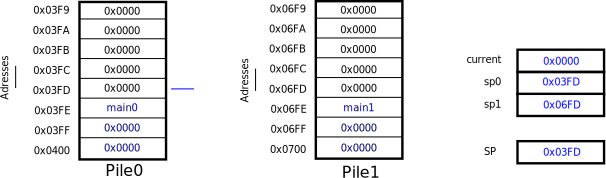
\includegraphics[width=\linewidth]{Figs/stack_ordonnanceur_init.png}
\caption{\label{stack_ordonnanceur_init} Etat des piles et des variables globales de l'ordonnanceur après la phase d'initialisation.}
\end{figure}

Ainsi, le seul travail de l'ordonnanceur va être de modifier le pointeur de pile entre la pile0 et la pile1. En effet, lorsqu'une interruption est levée, l'instruction INT sauvegarde le contexte sur la pile courante. La routine d'interruption de l'ordonnanceur change alors le pointeur de pile et déclenche un retour d'interruption qui a pour conséquence de dépiler un contexte depuis la pile du second programme. Le basculement de contexte est illustré sur la figure \ref{stack_ordonnanceur}.

\begin{figure}[htbp]
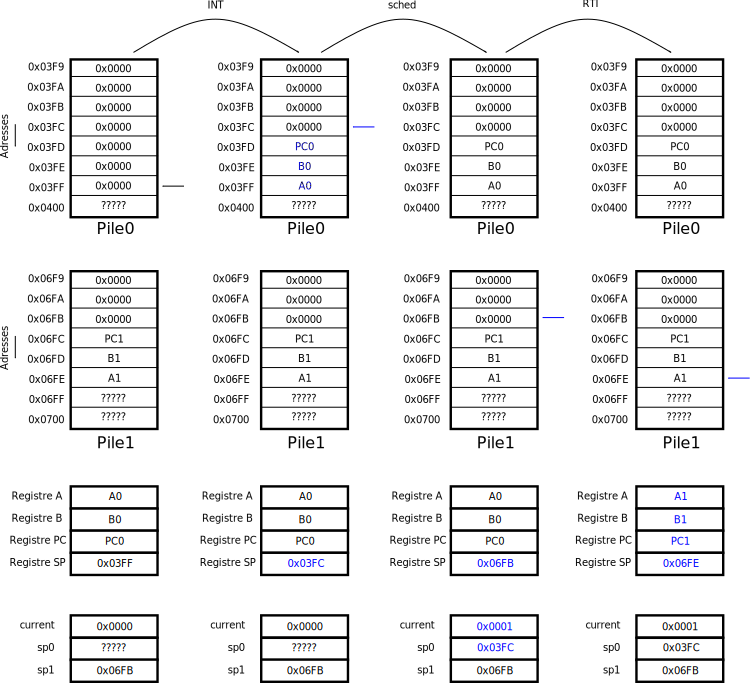
\includegraphics[width=\linewidth]{Figs/stack_ordonnanceur.png}
\caption{\label{stack_ordonnanceur} Illustration du changement de contexte lorsque l'ordonnanceur est réveillé par une interruption.}
\end{figure}

%\section{Interruptions, conflits, ..}




